% Reflow of the author v6 example at native paper size. No new image generation.
\begingroup
\fontfamily{qhv}\selectfont
\begin{tikzpicture}[x=1cm,y=1cm,
  every node/.style={inner sep=0pt},
  body/.style={font=\fontsize{7}{8.5}\selectfont,text=pInk,align=left},
  note/.style={font=\fontsize{7}{8.5}\selectfont,text=pMuted,align=left},
  head/.style={font=\bfseries\fontsize{8}{9.5}\selectfont,text=pInk,align=left},
  branch/.style={-{Stealth[length=1.3mm]},draw=pBlue,line width=.7pt},
  depth/.style={-{Stealth[length=1.3mm]},draw=pEvo,line width=.9pt},
  ghost/.style={draw=pEvo!25,line width=.6pt},
  candidateNode/.style={circle,draw=pEvo,fill=pLake!25,minimum size=.36cm,
    font=\bfseries\fontsize{7}{8}\selectfont,text=pInk},
  fail/.style={body,text=pRed,font=\bfseries\fontsize{7}{8.5}\selectfont},
  pass/.style={body,text=pEvo,font=\bfseries\fontsize{7}{8.5}\selectfont}]
\path[use as bounding box] (0,0) rectangle (13.7,7.70);

% The task is shared, not repeated in both searches.
\fill[pGoldWash,rounded corners=5pt] (0,4.84) rectangle (13.7,7.70);
\node[head,anchor=west] at (.18,7.40) {a\quad Task: image edits};
\node[body,anchor=north west,text width=3.45cm] at (.20,7.03)
  {Make a rainy night;\\keep the street layout\\and buildings unchanged.};
\node[pass,anchor=west] at (.20,5.81) {Human prefers A};
\node[fail,anchor=west] at (.20,5.43) {Scores favor B};
\node[note,anchor=west] at (.20,5.05) {Each edit is scored separately.};
\node[head] at (4.59,7.37) {Source};
\node[head] at (7.02,7.37) {A};
\node[head] at (10.88,7.37) {B};
\node[anchor=north] at (4.59,7.15) {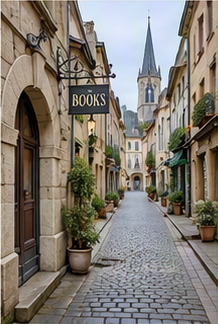
\includegraphics[width=1.38cm]{figures/teaser/source-street.png}};
\node[anchor=north] at (7.02,7.15) {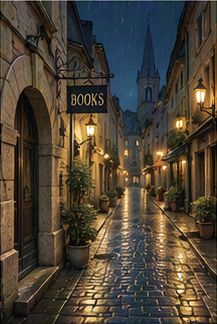
\includegraphics[width=1.38cm]{figures/teaser/edit-a.png}};
\node[anchor=north] at (10.88,7.15) {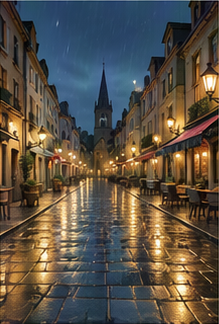
\includegraphics[width=1.38cm]{figures/teaser/edit-b.png}};
\node[body,anchor=west,text width=1.85cm] at (7.89,6.08) {Layout\\preserved};
\node[body,anchor=west,text width=1.75cm] at (11.74,6.08) {More vivid,\\but wider};

% The default setup branches across plausible, semantically distinct changes.
\fill[pBlueWash,rounded corners=5pt] (0,.02) rectangle (5.48,4.67);
\node[head,anchor=west] at (.18,4.38) {b\quad Default setup};
\node[body,anchor=west] at (.18,4.02) {Try a different direction};
\node[note] (seed) at (2.74,3.56) {Initial evaluation program};
\foreach \x/\n in {.93/1,2.74/2,4.55/3}{
  \node[candidateNode,draw=pBlue,fill=pBlue!18] (b\n) at (\x,2.89) {\n};
  \draw[branch] (2.74,3.35) .. controls (2.74,3.19) and (\x,3.21) .. (b\n.north);
  \draw[pBlue!30,line width=.5pt] (\x,1.12) -- (\x-.29,.79);
  \draw[pBlue!30,line width=.5pt] (\x,1.12) -- (\x+.29,.79);
  \draw[pBlue!30,fill=white] (\x-.29,.76) circle (.055);
  \draw[pBlue!30,fill=white] (\x+.29,.76) circle (.055);
}
\draw[branch,dashed] (b1) -- (b2);
\draw[branch,dashed] (b2) -- (b3);
\node[body,align=center,anchor=north,text width=1.66cm] at (.93,2.55)
  {\textbf{Compare\\source layout}\\[4pt]Wider street;\\not used\\in scoring};
\node[body,align=center,anchor=north,text width=1.66cm] at (2.74,2.55)
  {\textbf{Night / rain\\checks}\\[4pt]Night setting?\\Wet ground?};
\node[body,align=center,anchor=north,text width=1.66cm] at (4.55,2.55)
  {\textbf{Visual-defect\\checks}\\[4pt]Bad windows?\\Reflections?};
\node[fail] at (2.74,.36) {Still favors B after 1};

% Depth is a vertical spine. These are diagnostic revisions, not acceptances.
\fill[pEvoWash,rounded corners=5pt] (5.67,.02) rectangle (13.7,4.67);
\node[head,anchor=west] at (5.85,4.38) {c\quad IterEval: depth-first evaluator evolution};
\node[body,anchor=west] at (5.85,4.02) {Continue one direction: layout fidelity};
\node[note,anchor=west] at (5.85,3.65) {Initial evaluation program};
\coordinate (r) at (6.44,3.40);
\foreach \y/\n in {3.03/1,2.04/2,1.05/3}{
  \node[candidateNode] (c\n) at (6.44,\y) {\n};
  \draw[ghost] (6.44,\y+.40) .. controls (6.12,\y+.27) and (5.94,\y+.21) .. (5.94,\y+.04);
  \draw[ghost] (6.44,\y+.40) .. controls (6.76,\y+.27) and (6.94,\y+.21) .. (6.94,\y+.04);
  \draw[pEvo!30,fill=white] (5.94,\y) circle (.06);
  \draw[pEvo!30,fill=white] (6.94,\y) circle (.06);
  \draw[rounded corners=3pt,draw=pEvo!28,fill=white] (7.22,\y-.48) rectangle (13.51,\y+.42);
}
\draw[depth] (r) -- (c1);
\draw[depth] (c1) -- (c2);
\draw[depth] (c2) -- (c3);
\node[body,anchor=west] at (7.39,3.27) {\textbf{1\quad Detect layout changes}};
\node[body,anchor=west] at (7.39,2.97) {Changes detected, but unused in scoring.};
\node[fail,anchor=east] at (13.34,2.70) {Still favors B};
\node[body,anchor=west] at (7.39,2.28) {\textbf{2\quad Penalize layout changes}};
\node[body,anchor=west] at (7.39,1.98) {Penalty too small; error remains.};
\node[fail,anchor=east] at (13.34,1.71) {Still favors B};
\node[body,anchor=west] at (7.39,1.29) {\textbf{3\quad Scale the penalty by severity}};
\node[body,anchor=west] at (7.39,.99) {Larger layout changes, larger score penalties.};
\node[pass,anchor=east] at (13.34,.72) {Now favors A};
\node[note,anchor=west] at (5.86,.24) {Candidate acceptance and program inheritance are checked separately.};
\end{tikzpicture}
\endgroup
